% !TeX program = xelatex
% !TeX encoding = UTF-8
% !TeX TXS-program:compile = txs:///xelatex | txs:///xelatex
\documentclass[aspectratio=169, table, 12pt]{beamer}

% Preamble bersama seluruh slide mata kuliah ini.
% Dipanggil dari slides/sessionXX/sessionXX.tex tepat sesudah baris
% \documentclass[aspectratio=169, table, 12pt]{beamer}
% Paket tambahan yang hanya dibutuhkan satu sesi ditulis di berkas sesi itu.

\usepackage{colortbl}
\usepackage{xcolor}
\usepackage{listings}
\usepackage{tabularx}
\usepackage{booktabs}
\usepackage{tikz}
\usepackage{pgfplots}
\usepackage{fontspec}
\usepackage[english,bahasai]{babel}
\pgfplotsset{compat=1.18}
\usetikzlibrary{arrows.meta, positioning, calc, fit, shapes.geometric,
  shapes.multipart, backgrounds, matrix, chains, trees}

\makeatletter
\def\input@path{{../theme/}}
\makeatother
\graphicspath{{../theme/}{../../figures/}}
% Stub symlink Windows memakai tema cadangan sampai aset institusi tersedia.
\IfFileExists{../theme/beamerthemePradita.sty}{%
  \usetheme{Pradita}
}{%
  \usetheme{Madrid}
  \setmainfont{TeX Gyre Heros}
  \setsansfont{TeX Gyre Heros}
  \setbeamertemplate{navigation symbols}{}
}

\definecolor{praditagreen}{RGB}{37, 113, 71}
\setbeamercolor{structure}{fg=praditagreen}
\setbeamercolor{palette primary}{bg=praditagreen,fg=white}
\setbeamercolor{palette secondary}{bg=praditagreen!80!black,fg=white}
\setbeamercolor{palette tertiary}{bg=praditagreen!60!black,fg=white}
\setbeamerfont{frametitle}{size=\large}
\setbeamertemplate{caption}[numbered]

% Ukuran header mengikuti teks agar judul panjang tidak menabrak logo.
\setbeamercolor{frametitle}{bg=white,fg=black}
\setbeamertemplate{frametitle}{%
  \begin{beamercolorbox}[wd=\paperwidth,sep=0.2cm]{frametitle}
    \begin{minipage}[c]{0.77\paperwidth}
      \raggedright\fontsize{16}{18}\selectfont\bfseries\insertframetitle
      \ifx\insertframesubtitle\empty\else
        \par\small\mdseries\insertframesubtitle
      \fi
    \end{minipage}\hfill
    \begin{minipage}[c]{0.15\paperwidth}
      \IfFileExists{../theme/classFiles/logo_universitas.png}{%
        
\includegraphics[width=\linewidth]{../theme/classFiles/logo_universitas.png}%
      }{}
    \end{minipage}
  \end{beamercolorbox}
}
\setbeamertemplate{footline}{%
  \ifnum\value{framenumber}>1
    \begin{beamercolorbox}[wd=\paperwidth,ht=0.35cm,dp=0.15cm,
      leftskip=0.3cm,rightskip=0.3cm]{palette primary}
      \footnotesize\bfseries\insertframenumber/\inserttotalframenumber
      \hfill IT40513
    \end{beamercolorbox}
  \fi
}
\DeclareRobustCommand{\berkas}[1]{\path{#1}}

% Tema membuat garis tabel berwarna putih. Dikembalikan agar tabel terbaca.
\arrayrulecolor{black}
\setlength{\arrayrulewidth}{0.5pt}

\lstdefinelanguage{yaml}{
  basicstyle=\ttfamily\scriptsize,
  keywordstyle=\color{blue}\bfseries,
  commentstyle=\color{gray}\itshape,
  stringstyle=\color{red},
  showstringspaces=false,
  breaklines=true,
  frame=lines,
  numbers=none,
  backgroundcolor=\color{lightgray!10},
  tabsize=2,
  morecomment=[l]{\#}
}

\lstdefinelanguage{json}{
  basicstyle=\ttfamily\scriptsize,
  stringstyle=\color{red},
  commentstyle=\color{gray},
  breaklines=true,
  showstringspaces=false,
  tabsize=2,
  numbers=none,
  frame=lines,
  backgroundcolor=\color{lightgray!10},
  string=[s]{"}{"}
}

\lstdefinelanguage{bash}{
  keywords={},
  basicstyle=\ttfamily\scriptsize,
  ndkeywords={docker, kubectl, helm, curl, git, terraform},
  ndkeywordstyle=\color{purple}\bfseries,
  sensitive=true,
  commentstyle=\color{gray},
  numbers=none,
  breaklines=true,
  frame=lines,
  backgroundcolor=\color{lightgray!10},
  tabsize=2,
  comment=[l]{\#},
  showstringspaces=false
}

\lstdefinelanguage{http}{
  keywords={GET, POST, PUT, PATCH, DELETE, HEAD, OPTIONS, HTTP},
  basicstyle=\ttfamily\scriptsize,
  keywordstyle=\color{blue}\bfseries,
  sensitive=true,
  numbers=none,
  breaklines=true,
  frame=lines,
  backgroundcolor=\color{lightgray!10},
  tabsize=2,
  showstringspaces=false
}

\subtitle{IT40513 · Enterprise Architecture \& Digital Blueprint}
\author{\textbf{Alfa Yohannis}}


% Sampul membatasi judul di panel putih tema rujukan Pradita.
\setbeamertemplate{title page}{%
  \begin{tikzpicture}[remember picture,overlay]
    \node[anchor=north west,inner sep=0pt,text width=8.8cm]
      at ([xshift=1cm,yshift=-3.15cm]current page.north west) {%
        {\small\insertsubtitle\par}\vspace{0.25cm}
        \resizebox{8.8cm}{!}{\begin{minipage}{12cm}
          \raggedright\color{praditagreen}\bfseries\inserttitle
        \end{minipage}}
      };
    \node[anchor=south west,inner sep=0pt]
      at ([xshift=1cm,yshift=1.65cm]current page.south west)
      {\small\insertdate};
    \node[anchor=west,inner sep=0pt,text=white]
      at ([xshift=0.8cm,yshift=0.75cm]current page.south west)
      {\small\insertauthor};
  \end{tikzpicture}
}


% Batasi kedua dimensi gambar agar diagram bersama tetap berada pada slide.
\newsavebox{\eafigbox}
\newcommand{\eadiagram}[1]{%
  \sbox{\eafigbox}{\resizebox{0.94\textwidth}{!}{\input{#1}}}%
  \ifdim\dimexpr\ht\eafigbox+\dp\eafigbox\relax>0.64\textheight
    \resizebox{!}{0.64\textheight}{\usebox{\eafigbox}}%
  \else
    \usebox{\eafigbox}%
  \fi
}


\newcolumntype{Y}{>{\raggedright\arraybackslash}X}
\newcolumntype{L}[1]{>{\raggedright\arraybackslash}p{#1}}

% Font tema slide lebih lebar daripada font modul, sehingga sebagian kotak diagram bertumpuk.
% Lebar kotak dan jarak antarkotak dilonggarkan khusus di slide ini.
\makeatletter
\newcommand{\longgarkandiagram}[3]{%
  \tikzset{text width/.code={\def\tikz@text@width{#1}},
           every picture/.append style={x=#2, y=#3}}}
\makeatother

\title{\Huge Tata Kelola Arsitektur\\ \vspace{10pt} dan Praktik Lincah}
\date{Pertemuan 14}

\begin{document}

\frame{\titlepage}

\begin{frame}
  \frametitle{Isi Pertemuan}
  \vspace{14pt}
  \begin{columns}[t]
    \column{0.5\textwidth}
    {\small\tableofcontents[sections={1-4}]}

    \column{0.5\textwidth}
    {\small\tableofcontents[sections={5-7}]}
  \end{columns}
\end{frame}

\begin{frame}{\hfill}
  \centering
  \Huge{\textbf{Cetak biru sudah disetujui,\\mengapa proyek berikutnya\\tidak membukanya lagi?}}
\end{frame}

\section{Tujuan dan Konteks}

\begin{frame}{\hfill}
  \centering
  \Huge{\textbf{Tujuan dan Konteks}}
\end{frame}

\begin{frame}{{\Large Tujuan Pembelajaran}}
  \vspace{10pt}
  \begin{itemize}
    \item Merancang mekanisme tata kelola arsitektur: \textit{architecture board}, tinjauan kepatuhan,
          dispensasi, dan repositori.
    \item Membandingkan praktik EA (\textit{Enterprise Architecture}) tradisional dengan praktik yang
          lincah, termasuk tata kelola arsitektur di sektor publik.
    \item Mempresentasikan dan mempertahankan cetak biru transformasi digital di hadapan pemangku
          kepentingan.
  \end{itemize}
\end{frame}

\begin{frame}{{\Large Masalah: Disetujui, Lalu Disimpan}}
  \small
  \vspace{6pt}
  \begin{itemize}
    \item Direksi menyetujui cetak biru. Enam bulan kemudian proyek berjalan tanpa membukanya lagi.
    \item Misalkan unit pemasaran membeli aplikasi loyalitas yang menyimpan data pasien sendiri.
    \item Rumah sakit Bandung memperpanjang kontrak Sistem Informasi Manajemen Rumah Sakit (SIMRS) lama
          tanpa klausul migrasi.
    \item Vendor Medikara+ menambah satu koneksi langsung ke basis data SIMRS Depok.
    \item Tidak ada yang wajib bertanya, dan tidak ada yang berwenang menjawab.
  \end{itemize}
\end{frame}

\begin{frame}{{\Large Diagram Konsep Bab 14}}
  \centering
  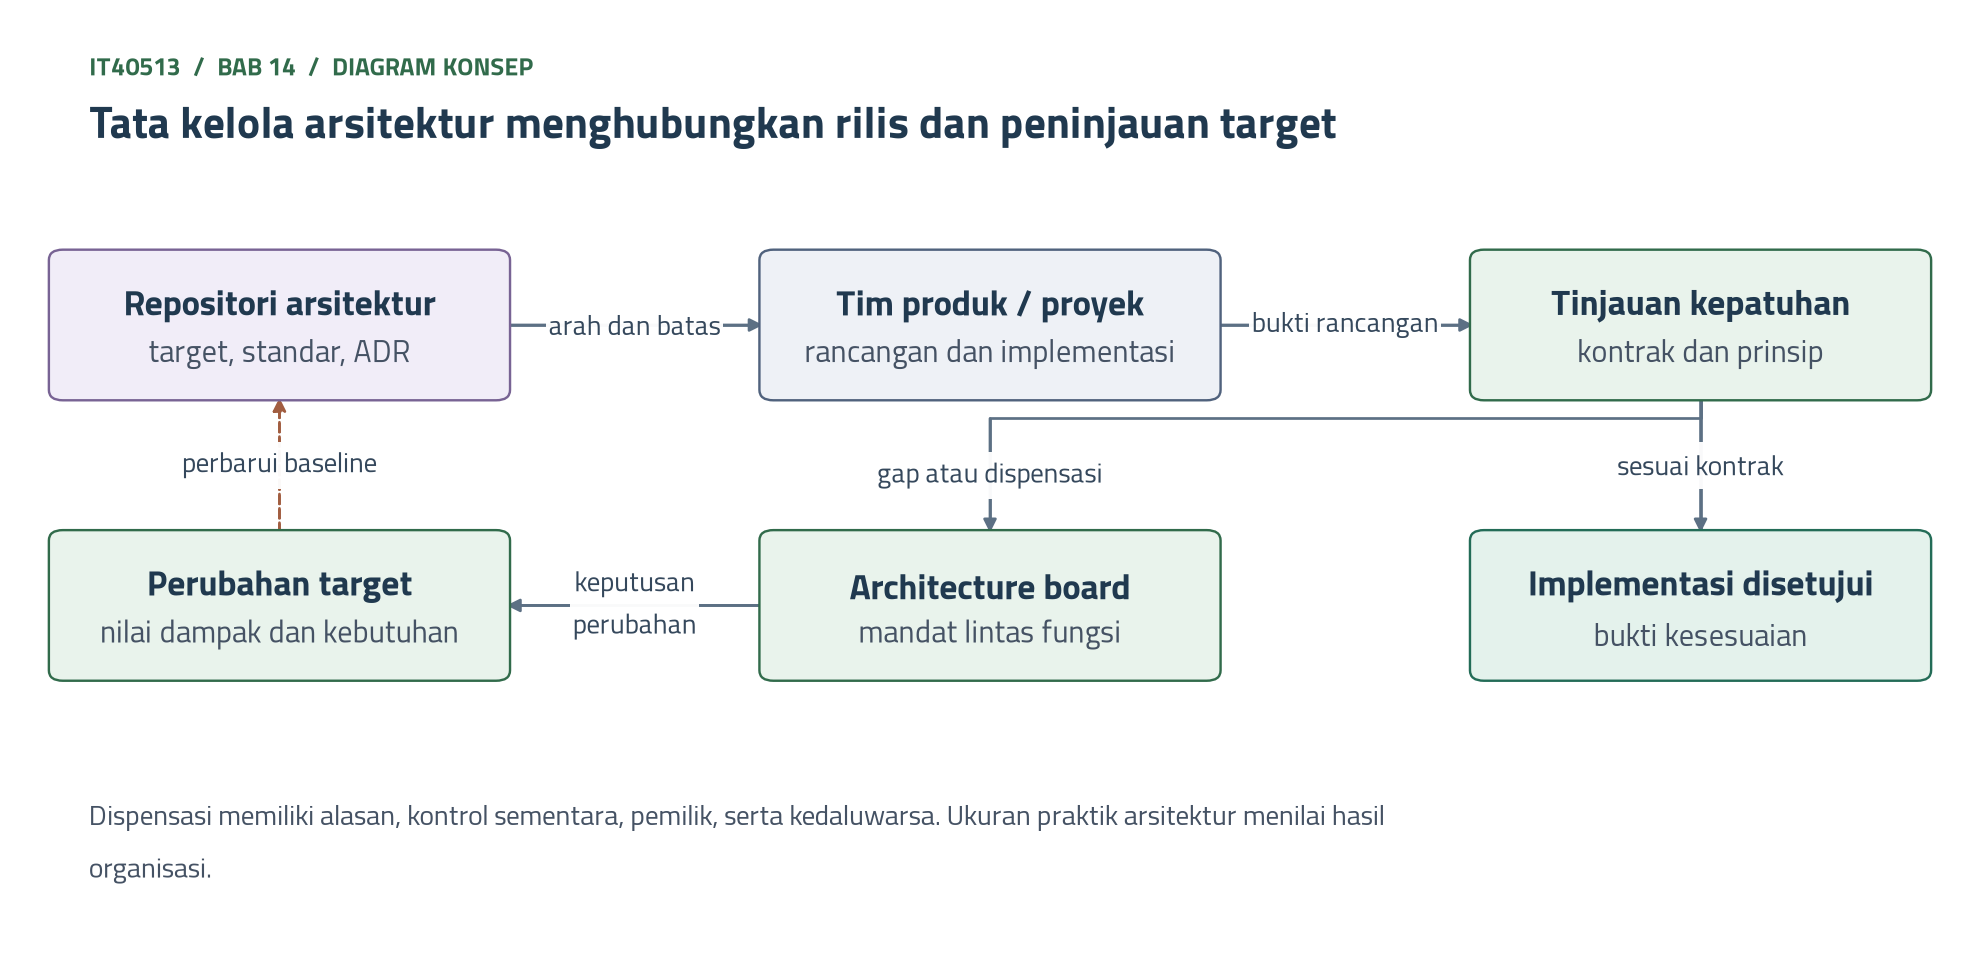
\includegraphics[width=0.96\textwidth,height=0.77\textheight,keepaspectratio]{../../figures/ch14-diagram-konsep.png}
  \label{fig:session14-ilustrasi-bab}
\end{frame}

\section{Implementasi dan Perubahan}

\begin{frame}{\hfill}
  \centering
  \Huge{\textbf{Implementasi\\dan Perubahan}}
\end{frame}

\begin{frame}{{\Large Fase G dan Fase H}}
  \small
  \vspace{6pt}
  \begin{itemize}
    \item Fase G dalam ADM (\textit{Architecture Development Method}), \textit{Implementation
          Governance}: memastikan proyek sesuai dengan arsitektur target.
    \item Alat utamanya kontrak arsitektur (\textit{architecture contract}) dan tinjauan kepatuhan.
    \item Fase H, \textit{Architecture Change Management}: menjaga arsitektur tetap relevan ketika
          bisnis, teknologi, dan regulasi berubah.
    \item \textit{Requirements Management}: mencatat dan menelusuri setiap kebutuhan sepanjang siklus.
  \end{itemize}
  \vspace{6pt}
  Analogi: konsultan pengawas menjalankan peran Fase G, prosedur perubahan gambar menjalankan peran
  Fase H.
\end{frame}

\begin{frame}{{\Large Dua Fase Terakhir ADM}}
  \centering
  \begin{figure}
    {\longgarkandiagram{3.3cm}{1cm}{0.98cm}%
    \resizebox{0.80\textwidth}{!}{\begin{tikzpicture}[
  font=\scriptsize,
  kotak/.style={draw, rounded corners, minimum height=0.95cm, text width=2.8cm,
                align=center, font=\scriptsize\bfseries},
  kecil/.style={draw, rounded corners, minimum height=0.7cm, text width=2.8cm,
                align=center, font=\scriptsize\bfseries},
  panah/.style={-{Stealth[length=2mm]}, thick}
]
  \node[kotak, fill=blue!8] (ef) at (0,0)
    {Fase E dan F\\{\tiny\mdseries peta jalan dan rencana migrasi}};
  \node[kotak, fill=orange!12] (g) at (4.3,0)
    {Fase G\\{\tiny\mdseries tata kelola implementasi: kontrak arsitektur dan tinjauan
    kepatuhan}};
  \node[kotak, fill=green!10] (hasil) at (8.6,0)
    {Solusi berjalan\\{\tiny\mdseries sesuai arsitektur target}};
  \node[kotak, fill=orange!12] (h) at (4.3,-3.0)
    {Fase H\\{\tiny\mdseries manajemen perubahan arsitektur}};
  \node[kotak, fill=praditagreen!15] (req) at (0,-3.0)
    {Requirements Management\\{\tiny\mdseries kebutuhan dicatat dan ditelusuri
    sepanjang siklus}};
  \node[kecil, fill=blue!8] (sederhana) at (8.6,-1.7)
    {Penyederhanaan\\{\tiny\mdseries manajemen perubahan biasa}};
  \node[kecil, fill=blue!8] (inkremental) at (8.6,-3.0)
    {Inkremental\\{\tiny\mdseries arsitektur diperbarui sebagian}};
  \node[kecil, fill=red!22] (ulang) at (8.6,-4.3)
    {Arsitektur ulang\\{\tiny\mdseries siklus ADM baru dari Fase A}};

  \draw[panah] (ef) -- (g);
  \draw[panah] (g) -- (hasil);
  \draw[panah] (g) -- (h);
  \draw[panah] (h.east) -- ++(0.55,0) |- (sederhana.west);
  \draw[panah] (h.east) -- (inkremental.west);
  \draw[panah] (h.east) -- ++(0.55,0) |- (ulang.west);
  \draw[dashed, thick, gray] (req) -- (h);
  \draw[dashed, thick, gray] (req) -- (ef);
  \draw[dashed, thick, gray] (req.north east) -- (g.south west);

  \node[font=\tiny, gray, anchor=west] at (4.4,-1.5) {permintaan perubahan};
  \node[font=\tiny, gray, align=center, anchor=north] at (4.3,-3.7)
    {pemicu: proyek, strategi bisnis,\\teknologi baru, dan regulasi};
\end{tikzpicture}
}}
    \caption{Fase G mengawal proyek menuju arsitektur target, sedangkan Fase H memilah permintaan
             perubahan menurut besar dampaknya}
  \end{figure}
\end{frame}

\begin{frame}{{\Large Kontrak Arsitektur}}
  \small
  \vspace{4pt}
  \begin{itemize}
    \item Kesepakatan tertulis antara fungsi arsitektur, sponsor proyek, dan tim pelaksana.
    \item Isinya: ruang lingkup solusi, prinsip dan standar wajib, titik tinjauan, dan cara menangani
          penyimpangan.
    \item Ditandatangani sebelum proyek mulai membangun.
    \item Misalkan kontrak Master Patient Index (MPI) memuat tiga titik tinjauan. Tinjauan pertama cukup
          mengubah dokumen rancangan.
    \item Misalkan platform integrasi memindahkan 23 koneksi dalam dua tahun, dengan target antara 8
          koneksi dalam 12 bulan.
  \end{itemize}
\end{frame}

\begin{frame}{{\Large Tiga Kelas Perubahan Arsitektur}}
  \footnotesize
  \begin{tabularx}{\textwidth}{L{2.5cm}YY}
    \hline
    \textbf{Kelas} & \textbf{Contoh di Medikara} & \textbf{Penanganan} \\
    \hline
    Penyederhanaan & Versi minimum PostgreSQL di katalog standar dinaikkan
      karena versi lama berhenti didukung & Manajemen perubahan biasa, lalu
      dicatat di repositori \\
    \hline
    Inkremental & Asuransi mitra baru memakai format klaim yang berbeda,
      sehingga arsitektur integrasi mitra perlu ditambah & Diperbarui
      sebagian lewat keputusan board, kadang dengan mengulang sebagian fase
      ADM \\
    \hline
    Arsitektur ulang & Misalkan Medikara mengakuisisi jaringan 25 klinik
      yang memakai sistem berbeda & Siklus ADM baru dimulai dari Fase A \\
    \hline
  \end{tabularx}

  \vspace{6pt}
  \small Manajemen perubahan TI mengatur sistem yang berjalan. Manajemen perubahan arsitektur mengatur
  arah: prinsip, standar, dan arsitektur target.
\end{frame}

\section{Board dan Tinjauan Kepatuhan}

\begin{frame}{\hfill}
  \centering
  \Huge{\textbf{Board dan\\Tinjauan Kepatuhan}}
\end{frame}

\begin{frame}{{\Large Architecture Board}}
  \small
  \vspace{4pt}
  \begin{itemize}
    \item Forum lintas fungsi yang diberi mandat mengambil keputusan arsitektur atas nama organisasi.
    \item Tanggung jawabnya: konsistensi, kepatuhan, dispensasi, perubahan arsitektur, dan pemakaian
          ulang komponen.
    \item TOGAF menyarankan empat atau lima anggota tetap, dan tidak lebih dari sepuluh.
    \item Mandat ditulis dalam piagam yang disahkan direksi. Tanpa itu, keputusan board hanya saran.
    \item Survei SAP LeanIX terhadap 360 arsitek: 92 persen menyatakan EA masih dipandang, seluruhnya
          atau sebagian, sebagai fungsi administratif TI.
  \end{itemize}
\end{frame}

\begin{frame}{{\Large Keanggotaan Board Medikara}}
  \small Misalkan Medikara menetapkan lima anggota tetap:
  \begin{itemize}
    \item Direktur Strategi dan Transformasi sebagai ketua.
    \item Direktur Pelayanan, yang mewakili dokter dan perawat.
    \item Direktur Keuangan, yang menanggung biaya integrasi.
    \item Kepala TI, yang menanggung operasi seluruh sistem.
    \item Kepala Arsitek \textit{Enterprise} sebagai sekretaris.
  \end{itemize}
  \vspace{4pt}
  Rapat rutin sebulan sekali selama dua jam. Board tidak memutuskan anggaran proyek. Keputusan investasi
  tetap di komite pengarah TI dan direksi.
\end{frame}

\begin{frame}{{\Large Daftar Periksa Kepatuhan}}
  \scriptsize
  \begin{tabularx}{\textwidth}{L{2.9cm}YY}
    \hline
    \textbf{Prinsip} & \textbf{Pertanyaan periksa} & \textbf{Bukti yang diminta} \\
    \hline
    PT1 Satu sumber data pasien & Apakah identitas pasien diambil dari MPI,
      bukan dibuat sendiri oleh aplikasi? & Diagram aliran data dan daftar
      tabel yang menyimpan identitas pasien \\
    \hline
    PT2 Akses berbasis peran dan tercatat & Apakah pengguna masuk lewat
      layanan identitas terpusat, dan apakah setiap akses ke rekam medis
      tercatat? & Rancangan otentikasi dan contoh catatan akses \\
    \hline
    PT3 Integrasi lewat antarmuka standar & Apakah pertukaran data klinis
      memakai HL7 FHIR lewat platform integrasi? & Katalog antarmuka proyek \\
    \hline
    PT4 Utamakan layanan bersama & Apakah fungsi yang sama sudah disediakan
      layanan bersama yang ada? & Hasil penelusuran katalog aplikasi \\
    \hline
    PT5 Data pasien dilindungi sejak rancangan & Apakah data pasien hanya
      dikumpulkan seperlunya dan disimpan di lokasi yang diizinkan? &
      Penilaian dampak pelindungan data dan rancangan penyimpanan \\
    \hline
  \end{tabularx}
\end{frame}

\begin{frame}{{\Large Enam Tingkat Kepatuhan}}
  \scriptsize
  \begin{tabularx}{\textwidth}{L{2.6cm}YY}
    \hline
    \textbf{Tingkat} & \textbf{Artinya} & \textbf{Contoh} \\
    \hline
    Tidak relevan (\textit{irrelevant}) & Solusi tidak bersinggungan dengan spesifikasi arsitektur &
      Aplikasi jadwal piket satpam dinilai terhadap standar data klinis \\
    \hline
    Konsisten (\textit{consistent}) & Sebagian fitur sesuai, ada yang belum dikerjakan, dan ada fitur
      lain di luar spesifikasi & Sistem laboratorium memakai FHIR, belum mencatat akses, dan menambah
      saluran pesan sendiri \\
    \hline
    Patuh (\textit{compliant}) & Sebagian belum dikerjakan, tetapi yang dikerjakan sesuai &
      Medikara+ memakai MPI untuk janji temu, telekonsultasi belum dipindah \\
    \hline
    Sesuai (\textit{conformant}) & Seluruh spesifikasi dikerjakan, ditambah fitur lain yang tidak sesuai &
      Memakai MPI sepenuhnya, tetapi menyalin data pasien ke \textit{spreadsheet} \\
    \hline
    Sesuai penuh (\textit{fully conformant}) & Spesifikasi dan solusi cocok sepenuhnya &
      Proyek MPI pada akhir uji terima \\
    \hline
    Tidak sesuai (\textit{non-conformant}) & Ada fitur yang dikerjakan bertentangan dengan spesifikasi &
      Aplikasi membuat nomor pasien sendiri \\
    \hline
  \end{tabularx}
\end{frame}

\begin{frame}{{\Large Dispensasi yang Cepat tetapi Terkendali}}
  \small
  \vspace{4pt}
  \begin{itemize}
    \item Dispensasi (\textit{dispensation}): izin resmi menyimpang dari arsitektur dalam waktu dan
          syarat tertentu.
    \item Dampak rendah diputuskan ketua board bersama kepala arsitek paling lama lima hari kerja.
    \item Dampak tinggi bila menyentuh data pasien, menambah koneksi di luar platform integrasi, atau
          biaya kembali patuh lebih dari Rp200 juta.
    \item Misalkan masa berlaku paling lama enam bulan, dan perpanjangan hanya satu kali.
    \item Tiga permintaan untuk prinsip yang sama dalam satu tahun: board mengusulkan perubahan
          arsitektur.
  \end{itemize}
\end{frame}

\begin{frame}{{\Large Alur Dispensasi Medikara}}
  \centering
  \begin{figure}
    {\longgarkandiagram{2.7cm}{1.45cm}{1cm}%
    \resizebox{!}{0.62\textheight}{\begin{tikzpicture}[
  font=\scriptsize,
  kotak/.style={draw, rounded corners, minimum height=0.95cm, text width=2.3cm,
                align=center, font=\scriptsize\bfseries},
  tanya/.style={draw, diamond, aspect=1.7, inner sep=1pt, align=center,
                font=\scriptsize\bfseries},
  panah/.style={-{Stealth[length=2mm]}, thick}
]
  \node[kotak, fill=blue!8] (rancangan) at (0,0)
    {Rancangan solusi\\{\tiny\mdseries diajukan tim proyek}};
  \node[kotak, fill=blue!8] (tinjau) at (3.1,0)
    {Tinjauan kepatuhan\\{\tiny\mdseries daftar periksa dari prinsip}};
  \node[tanya, fill=orange!12] (patuh) at (6.2,0) {Patuh?};
  \node[kotak, fill=green!10] (kontrak) at (9.3,0)
    {Kontrak arsitektur\\{\tiny\mdseries proyek lanjut}};
  \node[kotak, fill=orange!12] (minta) at (6.2,-2.0)
    {Permintaan dispensasi\\{\tiny\mdseries alasan, dampak, rencana kembali patuh}};
  \node[kotak, fill=blue!8] (cepat) at (3.1,-3.8)
    {Jalur cepat\\{\tiny\mdseries ketua dan kepala arsitek, paling lama 5 hari kerja}};
  \node[kotak, fill=orange!12] (putus) at (6.2,-3.8)
    {Keputusan\\{\tiny\mdseries tolak, atau setuju bersyarat dan berbatas waktu}};
  \node[kotak, fill=blue!8] (rapat) at (9.3,-3.8)
    {Rapat board\\{\tiny\mdseries dampak tinggi, dibahas di rapat bulanan}};
  \node[kotak, fill=praditagreen!15] (catat) at (6.2,-5.7)
    {Catatan tata kelola\\{\tiny\mdseries syarat, masa berlaku, tanggal tinjau}};
  \node[kotak, fill=green!10] (lanjut) at (9.3,-5.7)
    {Proyek lanjut\\{\tiny\mdseries dengan syarat yang dipantau}};
  \node[kotak, fill=red!22] (ulang) at (2.3,-5.7)
    {Usulan perubahan\\{\tiny\mdseries arsitektur lewat Fase H}};

  \draw[panah] (rancangan) -- (tinjau);
  \draw[panah] (tinjau) -- (patuh);
  \draw[panah] (patuh) -- node[above, font=\tiny] {ya} (kontrak);
  \draw[panah] (patuh) -- node[right, font=\tiny] {tidak} (minta);
  \draw[panah] (minta.west) -| node[above, pos=0.25, font=\tiny] {dampak rendah}
    (cepat.north);
  \draw[panah] (minta.east) -| node[above, pos=0.25, font=\tiny] {dampak tinggi}
    (rapat.north);
  \draw[panah] (cepat) -- (putus);
  \draw[panah] (rapat) -- (putus);
  \draw[panah] (putus) -- (catat);
  \draw[panah] (catat) -- (lanjut);
  \draw[panah] (catat) -- node[above, font=\tiny] {bila berulang} (ulang);
\end{tikzpicture}
}}
    \caption{Dampak rendah diputuskan cepat, dampak tinggi dibawa ke rapat board}
  \end{figure}
\end{frame}

\begin{frame}{{\Large Pengecualian dari Satu Sumber Data Pasien}}
  \begin{block}{Kasus Medikara Health}
    \small
    \begin{itemize}
      \item Misalkan Oktober 2027 Medikara memenangkan kontrak layanan untuk 3.500 karyawan, yang harus
            berjalan dalam delapan minggu.
      \item Platform vendor menyimpan data pasien sendiri, dan MPI baru dijadwalkan siap Maret 2028.
      \item Board memberi DSP-2027-07 yang berlaku sampai 30 April 2028, dengan empat syarat.
      \item Syarat: kunci MPI begitu siap, data harian ke SIMRS rujukan, bukan sumber laporan, serta
            ekspor HL7 FHIR dan penghapusan data dalam kontrak.
    \end{itemize}
  \end{block}
\end{frame}

\section{Repositori dan Kemampuan}

\begin{frame}{\hfill}
  \centering
  \Huge{\textbf{Repositori dan\\Kemampuan Arsitektur}}
\end{frame}

\begin{frame}{{\Large Isi Repositori Arsitektur Medikara}}
  \scriptsize
  \begin{tabularx}{\textwidth}{L{2.5cm}YL{2.3cm}L{2.7cm}}
    \hline
    \textbf{Bagian} & \textbf{Contoh isi} & \textbf{Pemelihara} & \textbf{Diperbarui} \\
    \hline
    Metamodel & Struktur folder Archi dan konvensi nama dari Bab 4 &
      Kurator repositori & Bila kerangka berubah \\
    \hline
    Kemampuan arsitektur & Piagam board, alur dispensasi, daftar peran &
      Kepala arsitek & Setiap tahun \\
    \hline
    Lanskap arsitektur & Model kondisi saat ini (C2), target (C3), dan
      transisi (C4) & Arsitek domain & Setiap kuartal dan setiap transisi
      selesai \\
    \hline
    Pustaka standar & Prinsip C1, katalog standar teknologi, profil HL7 FHIR
      & Arsitek teknologi & Setiap keputusan board \\
    \hline
    Pustaka referensi & Model referensi kesehatan dari BIZBOK, pola
      integrasi & Kepala arsitek & Bila ada rujukan baru \\
    \hline
    Catatan tata kelola & Kontrak arsitektur, hasil tinjauan, dispensasi,
      dan ADR & Sekretaris board & Setiap rapat atau keputusan \\
    \hline
    Repositori kebutuhan & Kebutuhan dari strategi, regulasi, dan proyek &
      Analis bisnis & Terus-menerus \\
    \hline
    Lanskap solusi & Rancangan solusi tiap proyek & Arsitek solusi & Setiap
      tinjauan proyek \\
    \hline
  \end{tabularx}
\end{frame}

\begin{frame}{{\Large Isi, Peran, dan Tim Arsitektur}}
  \small
  \vspace{6pt}
  \begin{itemize}
    \item Kotusev menelaah artefak EA di 27 organisasi dan menemukan 24 jenis artefak yang terbukti
          berguna.
    \item Isi repositori ditentukan oleh keputusan yang perlu didukung, bukan daftar lengkap jenis model.
    \item Keputusan board belum selesai sebelum repositori diperbarui.
    \item Empat peran: kepala arsitek \textit{enterprise}, arsitek domain, arsitek solusi, dan kurator
          repositori.
    \item Misalkan tim tujuh orang untuk sekitar 4.800 karyawan. Tim itu cukup bila pemeriksaan rutin
          diotomasi.
  \end{itemize}
\end{frame}

\begin{frame}{{\Large Model Praktik: Medikara Memilih Hibrida}}
  \centering
  \begin{figure}
    \resizebox{0.70\textwidth}{!}{\begin{tikzpicture}[
  font=\scriptsize,
  induk/.style={draw, rounded corners, minimum height=0.8cm, text width=2.9cm,
                align=center, font=\scriptsize\bfseries},
  unit/.style={draw, rounded corners, minimum height=0.6cm, text width=0.85cm,
               align=center, font=\tiny\bfseries},
  panah/.style={-{Stealth[length=2mm]}, thick}
]
  % Model terpusat.
  \node[font=\footnotesize\bfseries] at (0,1.0) {Terpusat};
  \node[induk, fill=praditagreen!15] (pusat1) at (0,0)
    {Tim EA pusat\\{\tiny\mdseries menyusun seluruh arsitektur}};
  \node[unit, fill=blue!8] (a1) at (-1.05,-1.6) {RS};
  \node[unit, fill=blue!8] (b1) at (0,-1.6) {Klinik};
  \node[unit, fill=blue!8] (c1) at (1.05,-1.6) {Apotek};
  \draw[panah] (pusat1) -- (a1);
  \draw[panah] (pusat1) -- (b1);
  \draw[panah] (pusat1) -- (c1);
  \node[font=\tiny, align=center, anchor=north] at (0,-2.05)
    {konsisten, tetapi lambat\\dan jauh dari unit};

  % Model terfederasi.
  \node[font=\footnotesize\bfseries] at (4.0,1.0) {Terfederasi};
  \node[induk, fill=gray!35] (pusat2) at (4.0,0)
    {Forum arsitek\\{\tiny\mdseries koordinasi tanpa mandat kuat}};
  \node[unit, fill=orange!12] (a2) at (2.95,-1.6) {RS};
  \node[unit, fill=orange!12] (b2) at (4.0,-1.6) {Klinik};
  \node[unit, fill=orange!12] (c2) at (5.05,-1.6) {Apotek};
  \draw[dashed, thick] (pusat2) -- (a2);
  \draw[dashed, thick] (pusat2) -- (b2);
  \draw[dashed, thick] (pusat2) -- (c2);
  \node[font=\tiny, align=center, anchor=north] at (4.0,-2.05)
    {dekat dengan unit, tetapi\\mudah menyimpang};

  % Model hibrida.
  \node[font=\footnotesize\bfseries] at (8.0,1.0) {Hibrida};
  \node[induk, fill=praditagreen!15] (pusat3) at (8.0,0)
    {Tim EA pusat\\{\tiny\mdseries prinsip, standar, repositori}};
  \node[unit, fill=green!10] (a3) at (6.95,-1.6) {RS};
  \node[unit, fill=green!10] (b3) at (8.0,-1.6) {Klinik};
  \node[unit, fill=green!10] (c3) at (9.05,-1.6) {Apotek};
  \draw[panah] (pusat3) -- (a3);
  \draw[panah] (pusat3) -- (b3);
  \draw[panah] (pusat3) -- (c3);
  \node[font=\tiny, align=center, anchor=north] at (8.0,-2.05)
    {standar dipegang pusat,\\keputusan harian di unit};
\end{tikzpicture}
}
    \caption{Tiga model praktik EA. Model hibrida memisahkan aturan bersama yang dipegang pusat dari
             keputusan harian yang diambil di unit}
  \end{figure}
  \vspace{-6pt}
  \small Tiap rumah sakit menunjuk penanggung jawab arsitektur, dan katalog standar hanya diubah lewat
  board.
\end{frame}

\section{Sektor Publik}

\begin{frame}{\hfill}
  \centering
  \Huge{\textbf{Tata Kelola Arsitektur\\di Sektor Publik}}
\end{frame}

\begin{frame}{{\Large Tiga Regulasi yang Membentuk Kerangka}}
  \scriptsize
  \begin{tabularx}{\textwidth}{L{2.8cm}Y}
    \hline
    \textbf{Regulasi} & \textbf{Isi yang relevan} \\
    \hline
    Perpres 95/2018 & Tim Koordinasi Sistem Pemerintahan Berbasis Elektronik (SPBE) Nasional bertanggung
      jawab kepada Presiden (Pasal 59). Koordinator SPBE di tiap instansi (Pasal 60 dan 61). Arsitektur
      SPBE Nasional lima tahun, direviu pada paruh waktu dan tahun terakhir (Pasal 8). \\
    \hline
    Permen PANRB 8/2026 & Evaluasi Kinerja Pemerintah Digital, mencabut Permen PANRB 59/2020 (Pasal 12).
      Penilaian mandiri oleh asesor internal (Pasal 5), lalu asesor eksternal (Pasal 6). Hasilnya indeks
      Pemerintah Digital (Pasal 7 dan 8). \\
    \hline
    Perpres 83/2025 & Komite Digital Pemerintah, lembaga nonstruktural di bawah Presiden (Pasal 1).
      Wakil Ketua I menangani tata kelola, termasuk Arsitektur Pemerintah Digital (Pasal 6). \\
    \hline
  \end{tabularx}

  \vspace{6pt}
  \small PANRB: Pendayagunaan Aparatur Negara dan Reformasi Birokrasi.
\end{frame}

\begin{frame}{{\Large Lapisan Tata Kelola Publik}}
  \centering
  \begin{figure}
    \resizebox{!}{0.59\textheight}{\begin{tikzpicture}[
  font=\scriptsize,
  lapis/.style={draw, rounded corners, minimum height=0.95cm, text width=2.1cm,
                align=center, font=\scriptsize\bfseries},
  isi/.style={draw, rounded corners, minimum height=0.95cm, text width=3.7cm,
              align=center, font=\scriptsize\bfseries}
]
  \node[font=\footnotesize\bfseries] at (4.0,0.95) {Sektor publik};
  \node[font=\footnotesize\bfseries] at (8.5,0.95) {Medikara Health};

  \node[lapis, fill=praditagreen!15] (l1) at (0,0) {Arah dan percepatan};
  \node[isi, fill=blue!8] (p1) at (4.0,0)
    {Komite Digital Pemerintah\\{\tiny\mdseries Perpres 83/2025, di bawah Presiden}};
  \node[isi, fill=green!10] (m1) at (8.5,0)
    {Direksi dan komite pengarah TI\\{\tiny\mdseries dibahas rinci di IT40813}};

  \node[lapis, fill=praditagreen!15] (l2) at (0,-1.35) {Koordinasi arsitektur};
  \node[isi, fill=blue!8] (p2) at (4.0,-1.35)
    {Tim Koordinasi SPBE Nasional\\{\tiny\mdseries Perpres 95/2018 Pasal 59, ketua
    menteri PANRB}};
  \node[isi, fill=green!10] (m2) at (8.5,-1.35)
    {\textit{Architecture board}\\{\tiny\mdseries piagam disahkan direksi}};

  \node[lapis, fill=praditagreen!15] (l3) at (0,-2.7) {Pelaksana di unit};
  \node[isi, fill=blue!8] (p3) at (4.0,-2.7)
    {Koordinator SPBE instansi\\{\tiny\mdseries Pasal 60 dan 61, ditetapkan pimpinan
    instansi}};
  \node[isi, fill=green!10] (m3) at (8.5,-2.7)
    {Arsitek domain dan tim proyek\\{\tiny\mdseries terikat kontrak arsitektur}};

  \node[lapis, fill=praditagreen!15] (l4) at (0,-4.05) {Pengukuran};
  \node[isi, fill=orange!12] (p4) at (4.0,-4.05)
    {Evaluasi Kinerja Pemerintah Digital\\{\tiny\mdseries Permen PANRB 8/2026,
    asesor internal dan eksternal}};
  \node[isi, fill=orange!12] (m4) at (8.5,-4.05)
    {Ukuran nilai EA\\{\tiny\mdseries dilaporkan ke direksi tiap kuartal}};

  \draw[dashed, gray, thick] (p1) -- (m1);
  \draw[dashed, gray, thick] (p2) -- (m2);
  \draw[dashed, gray, thick] (p3) -- (m3);
  \draw[dashed, gray, thick] (p4) -- (m4);
\end{tikzpicture}
}
    \caption{Lapisan tata kelola arsitektur di sektor publik dan padanannya di Medikara Health}
  \end{figure}
\end{frame}

\begin{frame}{{\Large Pelajaran bagi Organisasi Swasta}}
  \small
  \vspace{6pt}
  \begin{itemize}
    \item Arsitektur punya masa berlaku dan jadwal reviu. Cetak biru 2026 sampai 2030 direviu pada 2028
          dan 2030.
    \item Penilaian mandiri dipisahkan dari penilaian pihak lain.
    \item Koordinasi lintas unit membutuhkan mandat dari pimpinan tertinggi.
    \item Peringatan: indeks yang dipublikasikan mudah berubah menjadi tujuan.
  \end{itemize}
  \vspace{6pt}
  Analogi: uji berkala kendaraan angkutan. Kendaraan yang tidak pernah diuji pasti lebih berbahaya.
\end{frame}

\section{Praktik yang Lincah}

\begin{frame}{\hfill}
  \centering
  \Huge{\textbf{Praktik yang Lincah}}
\end{frame}

\begin{frame}{{\Large Arsitektur Disengaja dan yang Tumbuh}}
  \small
  \vspace{4pt}
  \begin{itemize}
    \item Open Agile Architecture Standard versi 2.0 terbit April 2026.
    \item \textit{Intentional architecture}: keputusan mahal diubah dan lintas tim, misalnya identitas
          pasien tunggal dan lokasi data.
    \item Arsitektur yang tumbuh (\textit{emergent architecture}): keputusan lokal yang murah diubah.
    \item \textit{Continuous architectural refactoring}: struktur tidak sehat diperbaiki sedikit demi
          sedikit pada setiap siklus.
    \item Pagar pembatas (\textit{guardrail}) seperti garis sempadan: isi kavling bebas selama tidak
          melewatinya.
  \end{itemize}
\end{frame}

\begin{frame}{{\Large EA Tradisional dan EA Lincah}}
  \scriptsize
  \begin{tabularx}{\textwidth}{L{2.4cm}YY}
    \hline
    \textbf{Aspek} & \textbf{Tradisional} & \textbf{Lincah} \\
    \hline
    Unit kerja & Cetak biru besar yang disusun sekali untuk beberapa tahun &
      Arsitektur yang disengaja untuk keputusan mahal, sisanya tumbuh bertahap \\
    \hline
    Artefak & Dokumen lengkap untuk semua domain & Artefak secukupnya: ADR,
      rancangan satu halaman, model yang dipakai \\
    \hline
    Waktu keputusan & Menunggu rapat terjadwal & Rutin diputuskan tim dalam
      pagar pembatas, pengecualian dibawa ke board \\
    \hline
    Peran arsitek & Penjaga gerbang di akhir proyek & Pendamping tim sejak
      awal, penyedia pola dan layanan bersama \\
    \hline
    Pemeriksaan kepatuhan & Tinjauan dokumen secara manual & Pemeriksaan
      otomatis untuk aturan yang dapat ditulis, tinjauan manual untuk penilaian \\
    \hline
    Umpan balik & Saat proyek selesai atau saat audit & Setiap siklus,
      lewat \textit{pipeline} dan tinjauan singkat \\
    \hline
  \end{tabularx}
\end{frame}

\begin{frame}{{\Large Board Tetap Ada, Antrean Berkurang}}
  \small
  \vspace{4pt}
  \begin{itemize}
    \item Tim produk Medikara+ bekerja dalam siklus dua minggu, sedangkan board rapat sebulan sekali.
    \item Misalkan tinjauan rancangan rata-rata menunggu 15 hari kerja.
    \item Sesudah PT1 sampai PT5 diperiksa otomatis, sekitar 70 persen perubahan lolos tanpa rapat.
    \item Sisanya masuk jalur cepat paling lama lima hari kerja, atau rapat board bila dampaknya tinggi.
    \item Misalkan konsolidasi SIMRS cukup empat keputusan disengaja: MPI, HL7 FHIR, identitas terpusat,
          dan region \textit{cloud} di Indonesia.
  \end{itemize}
\end{frame}

\begin{frame}{{\Large Pendalaman: Fitness Function}}
  \centering
  \begin{figure}
    \resizebox{0.76\textwidth}{!}{\begin{tikzpicture}[
  font=\scriptsize,
  kotak/.style={draw, rounded corners, minimum height=0.95cm, text width=2.2cm,
                align=center, font=\scriptsize\bfseries},
  panah/.style={-{Stealth[length=2mm]}, thick}
]
  \node[kotak, fill=blue!8] (ubah) at (0,0)
    {Perubahan\\{\tiny\mdseries kode atau konfigurasi}};
  \node[kotak, fill=blue!8] (uji) at (2.9,0)
    {Build dan uji\\{\tiny\mdseries \textit{pipeline} CI}};
  \node[kotak, fill=orange!12] (fungsi) at (5.8,0)
    {\textit{Fitness function}\\{\tiny\mdseries periksa standar teknologi}};
  \node[kotak, fill=green!10] (lolos) at (9.2,0.95)
    {Lolos\\{\tiny\mdseries boleh digabung}};
  \node[kotak, fill=red!22] (gagal) at (9.2,-0.95)
    {Gagal\\{\tiny\mdseries diblokir}};
  \node[kotak, fill=praditagreen!15] (catatan) at (5.8,-2.5)
    {Catatan dispensasi\\{\tiny\mdseries nomor dan tanggal berakhir}};
  \node[kotak, fill=blue!8] (board) at (9.2,-2.5)
    {\textit{Architecture board}\\{\tiny\mdseries menilai pengecualian}};

  \draw[panah] (ubah) -- (uji);
  \draw[panah] (uji) -- (fungsi);
  \draw[panah] (fungsi.east) -- ++(0.45,0) |- (lolos.west);
  \draw[panah] (fungsi.east) -- ++(0.45,0) |- (gagal.west);
  \draw[panah] (gagal) -- node[right, font=\tiny] {eskalasi} (board);
  \draw[panah, dashed] (board) -- node[below, font=\tiny] {dispensasi dicatat}
    (catatan);
  \draw[panah, dashed] (catatan) -- node[left, font=\tiny] {dibaca} (fungsi);
  \node[font=\tiny, gray, anchor=east] at (7.75,0.75) {sesuai standar};
  \node[font=\tiny, gray, anchor=east] at (7.75,-0.75) {ada pelanggaran};
\end{tikzpicture}
}
    \caption{\textit{Fitness function} menilai perubahan dan meneruskan pelanggaran ke board}
  \end{figure}
  \vspace{-6pt}
  \small Pada contoh 30 Oktober 2027, 3 komponen melanggar. Pada 15 Mei 2028, DSP-2027-07 sudah berakhir
  dan pelanggaran naik menjadi 4.
\end{frame}

\section{Nilai, Aktivitas, dan Penutup}

\begin{frame}{\hfill}
  \centering
  \Huge{\textbf{Nilai, Aktivitas,\\dan Penutup}}
\end{frame}

\begin{frame}{{\Large Ukuran Aktivitas dan Ukuran Hasil}}
  \small
  \vspace{4pt}
  \begin{itemize}
    \item Ukuran aktivitas: jumlah diagram, rapat, dan halaman. Mudah dikumpulkan, mudah digelembungkan.
    \item Ukuran hasil: perubahan pada organisasi, misalnya identitas ganda dan koneksi
          \textit{point-to-point}.
    \item Lange dkk., 133 praktisi: keterlekatan dalam organisasi menjadi konstruk sentral, sedangkan
          kepuasan terhadap EA tidak menentukan.
    \item Tamm dkk.: EA memberi nilai lewat empat pemungkin manfaat.
    \item Waktu keputusan yang memendek baru bermakna bila pemakaian MPI ikut naik.
  \end{itemize}
\end{frame}

\begin{frame}{{\Large Ukuran Nilai Praktik EA Medikara}}
  \scriptsize
  \begin{tabularx}{\textwidth}{L{2.5cm}YY}
    \hline
    \textbf{Tingkat} & \textbf{Ukuran} & \textbf{Tujuan bisnis yang dilayani} \\
    \hline
    Pemakaian & Persentase proyek baru yang ditinjau sebelum kontrak vendor
      ditandatangani & Arsitektur ikut menentukan keputusan, bukan hanya mencatatnya \\
    \hline
    Manfaat proyek & Median hari kerja dari permintaan sampai keputusan
      arsitektur & Proyek tidak tertahan oleh tata kelola \\
    \hline
    Manfaat proyek & Persentase proyek baru yang memakai MPI dan layanan
      identitas terpusat & Satu Pasien, Satu Rekam Medis; kontrol akses \\
    \hline
    Manfaat organisasi & Jumlah koneksi \textit{point-to-point} yang masih aktif & Biaya integrasi turun \\
    \hline
    Manfaat organisasi & Persentase identitas pasien ganda di MPI &
      Layanan terintegrasi lintas fasilitas \\
    \hline
    Aktivitas (tidak dipakai) & Jumlah diagram, jumlah rapat, jumlah
      halaman dokumen & Tidak terhubung ke tujuan bisnis mana pun \\
    \hline
  \end{tabularx}

  \vspace{6pt}
  \small Misalkan laporan kuartal ketiga 2027: koneksi \textit{point-to-point} turun dari 23 menjadi 15.
\end{frame}

\begin{frame}{{\Large Aktivitas: Tata Kelola dan Presentasi Akhir}}
  \small
  \begin{itemize}
    \item Rumuskan mandat dan keanggotaan \textit{architecture board}.
    \item Turunkan daftar periksa kepatuhan dari prinsip C1.
    \item Rancang alur dispensasi: kriteria, jalur cepat, batas waktu, dan masa berlaku.
    \item Tetapkan pemeliharaan repositori dan tiga sampai lima ukuran nilai EA.
    \item Susun presentasi C1 sampai C4, lalu latih tanya jawab.
  \end{itemize}
  \footnotesize Peran: analis bisnis, analis teknologi, pemodel, koordinator. Luaran: tonggak C4.
  Lima kriteria rubrik, masing-masing 20 persen.
  Rubrik: \berkas{sources/chapter14/rubrik-presentasi-c4.md}.
\end{frame}

\begin{frame}{{\Large Ringkasan}}
  \small
  \vspace{4pt}
  \begin{itemize}
    \item Fase G mengawal proyek lewat kontrak dan tinjauan. Fase H memilah perubahan menurut dampaknya.
    \item Board yang efektif kecil, melibatkan bisnis, dan bekerja berdasarkan piagam yang disahkan
          direksi.
    \item Dispensasi bersyarat, berbatas waktu, dan tercatat.
    \item Praktik yang lincah menjaga tata kelola agar tidak menjadi antrean.
    \item Cetak biru bernilai sejauh ia dipakai untuk memutuskan.
  \end{itemize}
\end{frame}

\begin{frame}{{\Large Latihan}}
  \small
  \vspace{6pt}
  \begin{itemize}
    \item \textbf{Latihan 1: Merancang Alur Dispensasi.} Nilai dampak, tentukan jalur, syarat, masa
          berlaku, dan pemicu Fase H.
    \item \textbf{Latihan 2: Membandingkan Architecture Board dan Tim Koordinasi SPBE.} Bandingkan tujuh
          aspek dari dokumen publik satu instansi.
    \item \textbf{Latihan 3: Memilih Ukuran Nilai Praktik EA.} Pilih tiga ukuran hasil, lalu jelaskan
          mengapa jumlah diagram bukan ukuran yang baik.
  \end{itemize}
\end{frame}

\begin{frame}{{\Large Bacaan dan Berkas Pendukung}}
  \small
  \vspace{6pt}
  \begin{itemize}
    \item \href{https://www.opengroup.org/togaf}{The TOGAF Standard, 10th Edition (2025 Update)}
    \item \href{https://peraturan.bpk.go.id/Details/96913/perpres-no-95-tahun-2018}{Peraturan Presiden Nomor 95 Tahun 2018 tentang Sistem Pemerintahan Berbasis Elektronik}
    \item \href{https://peraturan.bpk.go.id/Details/329002/perpres-no-83-tahun-2025}{Peraturan Presiden Nomor 83 Tahun 2025 tentang Komite Percepatan Transformasi Digital Pemerintah}
    \item \berkas{sources/chapter14/README.md}
  \end{itemize}
\end{frame}

\end{document}
